\chapter{Plotting data}
\label{ch:plotting}

A picture says more than a thousand words and nowhere is this more
true than in statistics. So before we explore the more quantitative
aspects of data analysis, it is useful to \emph{visualise} the data.
Consider, for example, the following four bivariate datasets
(Anscombe's quartet\footnote{Anscombe, F.J., 1973. Graphs in
  statistical analysis. \emph{The American statistician}, 27(1),
  pp.17-21.}):\medskip

\noindent\begin{minipage}[t][][b]{.6\textwidth}
  \begin{tabular}{cc|cc|cc|cc}
    \multicolumn{2}{c}{I} & \multicolumn{2}{c}{II} &
    \multicolumn{2}{c}{III} & \multicolumn{2}{c}{IV} \\
    $x$ & $y$ & $x$ & $y$ & $x$ & $y$ & $x$ & $y$ \\ \hline
    10.0 & 8.04 & 10.0 & 9.14 & 10.0 & 7.46 & 8.0 & 6.58 \\
    8.0 & 6.95 & 8.0 & 8.14 & 8.0 & 6.77 & 8.0 & 5.76 \\
    13.0 & 7.58 & 13.0 & 8.74 & 13.0 & 12.74 & 8.0 & 7.71 \\
    9.0 & 8.81 & 9.0 & 8.77 & 9.0 & 7.11 & 8.0 & 8.84 \\
    11.0 & 8.33 & 11.0 & 9.26 & 11.0 & 7.81 & 8.0 & 8.47 \\
    14.0 & 9.96 & 14.0 & 8.10 & 14.0 & 8.84 & 8.0 & 7.04 \\
    6.0 & 7.24 & 6.0 & 6.13 & 6.0 & 6.08 & 8.0 & 5.25 \\
    4.0 & 4.26 & 4.0 & 3.10 & 4.0 & 5.39 & 19.0 & 12.50 \\
    12.0 & 10.84 & 12.0 & 9.13 & 12.0 & 8.15 & 8.0 & 5.56 \\
    7.0 & 4.82 & 7.0 & 7.26 & 7.0 & 6.42 & 8.0 & 7.91 \\
    5.0 & 5.68 & 5.0 & 4.74 & 5.0 & 5.73 & 8.0 & 6.89 \\
  \end{tabular}
\end{minipage}
\begin{minipage}[t][][t]{.4\textwidth}
  \captionof{table}{Anscombe's quartet of bivariate data pairs.}
  \label{tab:anscombe}
\end{minipage}\medskip

For all four datasets (I -- IV):

\begin{itemize}\label{pg:anscombe}
\item the mean (see chapter~\ref{ch:summary-statistics}) of $x$ is 9
\item the variance (see chapter~\ref{ch:summary-statistics}) of $x$ is 11
\item the mean of $y$ is 7.50
\item the variance of $y$ is 4.125
\item the correlation coefficient (see chapter~\ref{ch:regression})
  between $x$ and $y$ is 0.816
\item the best fit line (see chapter~\ref{ch:regression}) is given by $y =
  3.00 + 0.500 x$
\end{itemize}

So from a numerical point of view, it would appear that all four
datasets are identical. However, when we visualise the data as
bivariate scatter plots, they turn out to be very different:\medskip

\noindent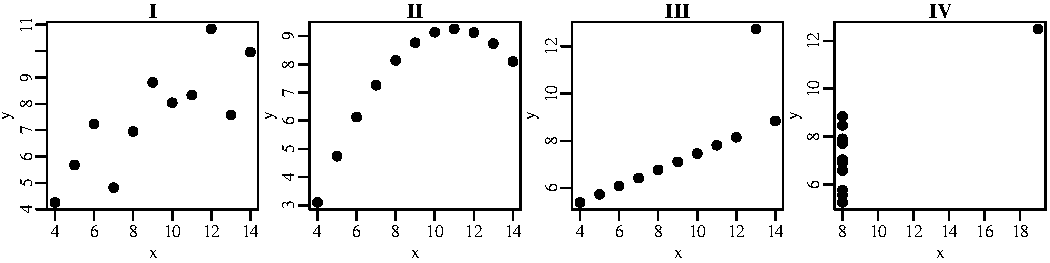
\includegraphics[width=\textwidth]{../figures/anscombe.pdf}
\begingroup
\captionof{figure}{Anscombe's quartet shown as bivariate scatter
  plots.\medskip}\label{fig:anscombe}
\endgroup

Bivariate scatter plots are just one way to visualise analytical data.
Many other graphical devices exist, each of which is appropriate for a
particular type of data. The following sections of this chapter will
introduce a number of these data types, and the associated plots.

\section{Categorical data}
\label{sec:categorical}

Categorical data take one of a limited number of values, assigning
each `object' to a particular class or category. Geological examples
of categorical data are:

\begin{itemize}
\item rock types in a mapping area;
\item animal species in a bone bed;
\item the modal composition of a thin section.
\end{itemize}

Consider, for example, the following 41 clast counts:

\begin{center}
  \begin{tabular}{cccc}
    granite & basalt & gneiss & quartzite \\ \hline
    10 & 5 & 6 & 20  
  \end{tabular}
\end{center}

A bar chart is the natural way to visualise these data:\medskip

\noindent\begin{minipage}[t][][b]{.4\textwidth}
  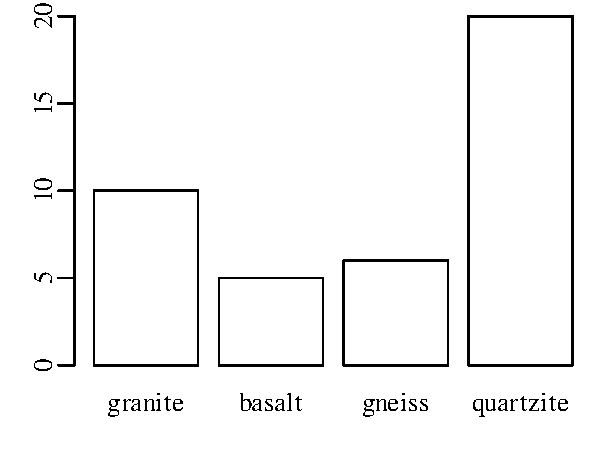
\includegraphics[width=\textwidth]{../figures/clasts.pdf}
\end{minipage}
\begin{minipage}[t][][t]{.6\textwidth}
  \captionof{figure}{Bar chart of clast counts. The vertical axis
    labels the number of objects counted in each category. The order
    of the categories along the horizontal axis is completely
    arbitrary and can be changed without loss of information.}
  \label{fig:clasts}
\end{minipage}

\section{Count data}
\label{sec:counts}

Count data are closely related to categorical data. Geological
examples of this type of data include:

\begin{itemize}
\item the annual number of earthquakes that exceed a certain
  magnitude;
\item the number of gold chips found in a panning session;
\item the number of dry wells in a wildcat drilling survey.
\end{itemize}

The crucial difference between count data and categorical data is that
the order of the categories matters for the count data, whereas it
does not for categorical data.  As an example, consider the number of
earthquakes of magnitude 5.0 or greater between 1917 and 2016:

\noindent\begin{minipage}[t][][b]{.4\textwidth}
  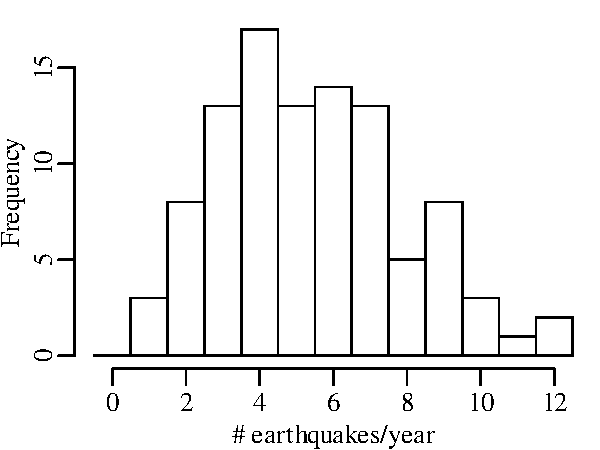
\includegraphics[width=\textwidth]{../figures/declusteredquakesperyear.pdf}
\end{minipage}
\begin{minipage}[t][][t]{.6\textwidth}
  \captionof{figure}{Histogram of magnitude $\geq{5.0}$ earthquakes per
    year between 1917 and 2016. The vertical axis labels the number of
    years. The horizontal axis shows the number of earthquakes. In
    contrast with Figure~\ref{fig:clasts}, the order of the four
    categories along the horizontal axis matters and cannot be changed
    without loss of information. Categorical data whose order matters
    are also known as \emph{ordinal} data.}
  \label{fig:quakecounts}
\end{minipage}

\section{Continuous data}
\label{sec:continuous}

Not all geological or geophysical measurements take integer values.
Many are free to take on any decimal value. A few examples of such
continuous data are:

\begin{itemize}
\item the magnitude of earthquakes;
\item the spontaneous electrical potential between geological strata;
\item the density of minerals;
\item the porosity of a sedimentary rock.
\end{itemize}

Consider the following dataset of pH measurements in 20~samples of
rain water:

\begin{center}
6.2, 4.4, 5.6, 5.2, 4.5, 5.4, 4.8, 5.9, 3.9, 3.8, 5.1, 4.1, 5.1, 5.5,
5.1, 4.6, 5.7, 4.6, 4.6, 5.6
\end{center}

These values can be collected into bins and plotted as a histogram,
just like the count data in section~\ref{sec:counts}. However this
binning exercise poses two practical problems.

\subsection*{i. How many bins should we use, and how wide should they be?}

The number of bins strongly affects the appearance of a histogram:

\noindent\begin{minipage}[t][][b]{.5\textwidth}
  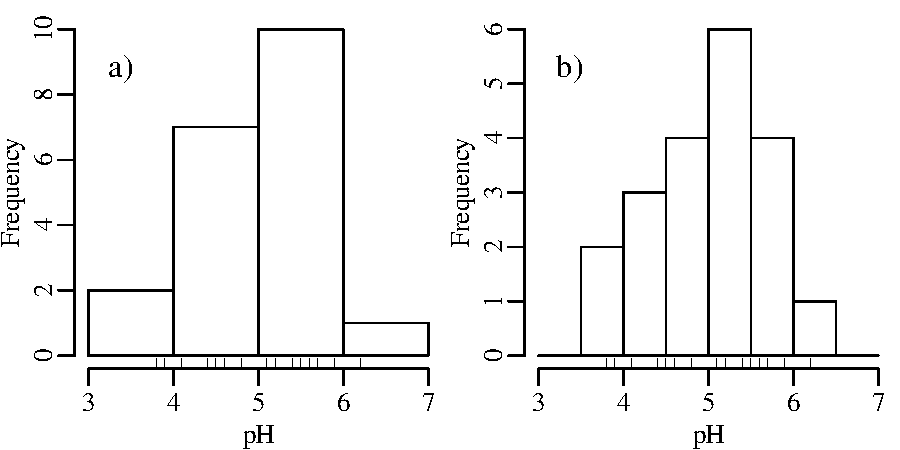
\includegraphics[width=\textwidth]{../figures/binwidth.pdf}\medskip
\end{minipage}
\begin{minipage}[t][][t]{.5\textwidth}
  \captionof{figure}{ Two histograms of the same pH data, with the
    individual measurements marked as vertical ticks underneath. This
    is also known as a \emph{rug plot}, and allows us to better assess
    the effect of bin width on the appearance of histograms.
    Histogram a) uses a bin width of 1~pH unit whereas histogram b)
    uses a bin width of 0.5~pH units. The two histograms look
    considerably different and it is not immediately clear which
    choice of bin width is best.}
  \label{fig:binwidth}
\end{minipage}

A number of rules of thumb are available to choose the optimal number
of bins. For example, \texttt{Excel} uses a simple square root rule:

\begin{equation}
  \mbox{\#{bins} = } \sqrt{n}
\end{equation}

\noindent where $n$ is the number of observations (i.e. $n = 20$ for
the pH example). \texttt{R} uses Sturges' Rule:

\begin{equation}
  \mbox{\#{bins} = } \log_2(n) + 1
\end{equation}

\noindent however no rule of thumb is optimal in all situations.

\subsection*{ii. Where to place the bins?}

Even when the number of bins has been fixed, just shifting them
slightly to the left or to the right can have a significant effect on
the appearance of the histogram. For example:

\noindent\begin{minipage}[t][][b]{.5\textwidth}
  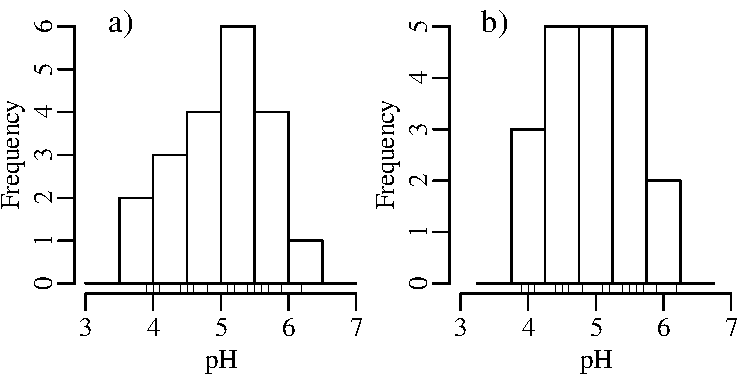
\includegraphics[width=\textwidth]{../figures/binpos.pdf}\medskip
\end{minipage}
\begin{minipage}[t][][t]{.5\textwidth}
  \captionof{figure}{Two histograms of the pH data whose bin widths
    are the same, but whose bins have been offset by 0.25 pH units.
    This arbitrary decision strongly affects the appearance of the
    histogram.}
  \label{fig:binpos}
\end{minipage}
  
To solve the bin placement problem, let us explore a variant of the
ordinary histogram that is constructed as follows:

\begin{enumerate}
\item Rank the measurements from low to high along a line.
\item Place a rectangular `box' on top of each measurement.
\item Stack the boxes to create one connected line.
\end{enumerate}

\noindent\begin{minipage}[t][][b]{.3\textwidth}
  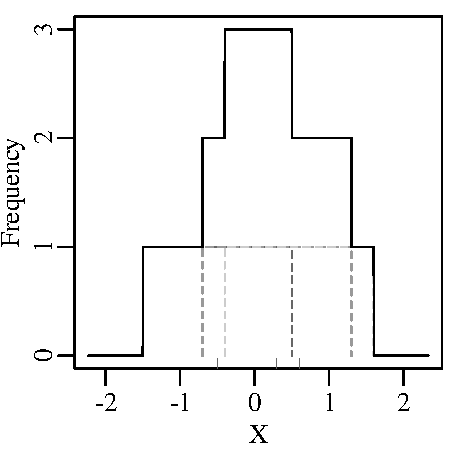
\includegraphics[width=\textwidth]{../figures/rectKDE.pdf}
\end{minipage}
\begin{minipage}[t][][t]{.7\textwidth}
  \captionof{figure}{The rug plot along the bottom axis represents
    three data points. The grey dashed lines mark rectangular boxes
    (`kernels') that are centred around each of these data points. The
    black step function is obtained by taking the sum of these
    boxes. This procedure removes the need to choose bin locations.}
  \label{fig:rectangles}
\end{minipage}

Normalising the area under the resulting curve produces a so-called
Kernel Density Estimate (KDE). The mathematical definition of this
function is:

\begin{equation}
  KDE(x) = \frac{1}{nh} \sum\limits_{i=1}^{n} K\!\left(\frac{x-x_i}{h}\right)
\end{equation}

\noindent where $x_i$ is the $i$\textsuperscript{th} measurement (out
of $n$), $h$ is the `bandwidth' of the kernel density estimator, and
$K(u)$ is the `kernel' function. For the rectangular kernel:

\begin{equation}
  K(u) = 1/2 \mbox{~if~}|u| \leq 1, \mbox{~and~} K(u) = 0 \mbox{~otherwise}
\end{equation}

Applying this method to the pH data:

\noindent\begin{minipage}[t][][b]{.3\textwidth}
  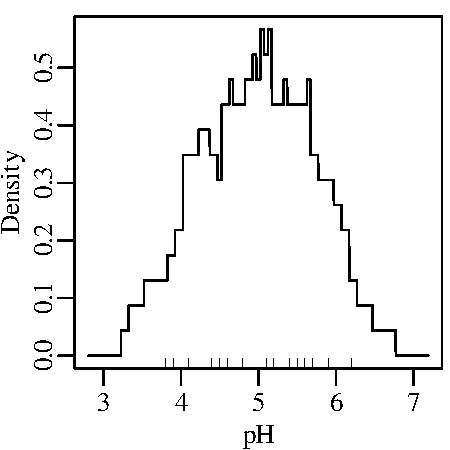
\includegraphics[width=\textwidth]{../figures/pHrectKDE.pdf}
\end{minipage}
\begin{minipage}[t][][t]{.7\textwidth}
  \captionof{figure}{Rectangular KDE of the pH data, constructed using
    the same procedure as shown in Figure~\ref{fig:rectangles}. The
    area under this curve has been normalised to unity.}
  \label{fig:pHrectKDE}
\end{minipage}

Instead of a rectangular kernel, we could also use triangles to
construct the KDE curve, or any other (symmetric) function. One
popular choice is the Gaussian function:

\begin{equation}
  K(u) = \frac{1}{\sqrt{2\pi}}\exp\!\left[-\frac{u^2}{2}\right]
  \label{eq:gaussiankernel}
\end{equation}

\noindent which produces a continuous KDE function:\medskip

\noindent\begin{minipage}[t][][b]{.3\textwidth}
  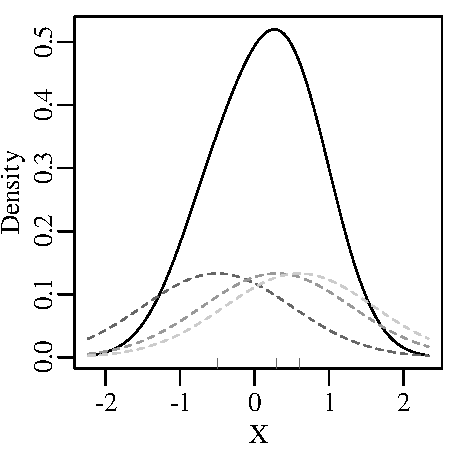
\includegraphics[width=\textwidth]{../figures/gaussKDE.pdf}
\end{minipage}
\begin{minipage}[t][][t]{.7\textwidth}
  \captionof{figure}{Using a Gaussian kernel instead of a rectangular
    kernel on the three data points of Figure~\ref{fig:rectangles}.
    This produces a smooth KDE.}
\end{minipage}

Using the Gaussian kernel to plot the pH data:\medskip

\noindent\begin{minipage}[t][][b]{.3\textwidth}
  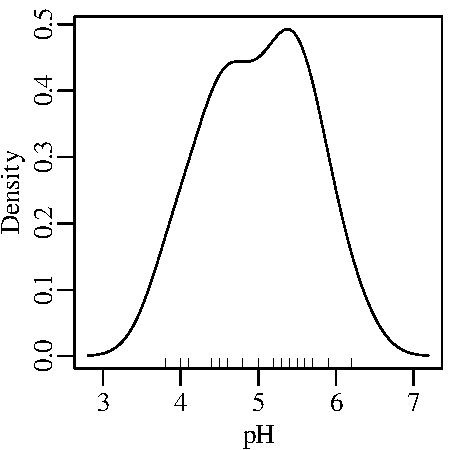
\includegraphics[width=\textwidth]{../figures/pHgaussKDE.pdf}\medskip
\end{minipage}
\begin{minipage}[t][][t]{.7\textwidth}
  \captionof{figure}{Gaussian KDE of the pH data. The continuous curve
    does more justice to the continuous data than the discrete step
    function of Figures~\ref{fig:binwidth}, \ref{fig:binpos} or
    \ref{fig:pHrectKDE}.}
  \label{fig:pHgaussKDE}
\end{minipage}

Although kernel density estimation solves the bin placement problem,
it is not entirely free of design decisions. The bandwidth $h$ of a
KDE fulfils a similar role as the bin width of a histogram. Changes in
$h$ affect the \emph{smoothness} of the KDE curve:\medskip

\noindent\begin{minipage}[t][][b]{.55\textwidth}
  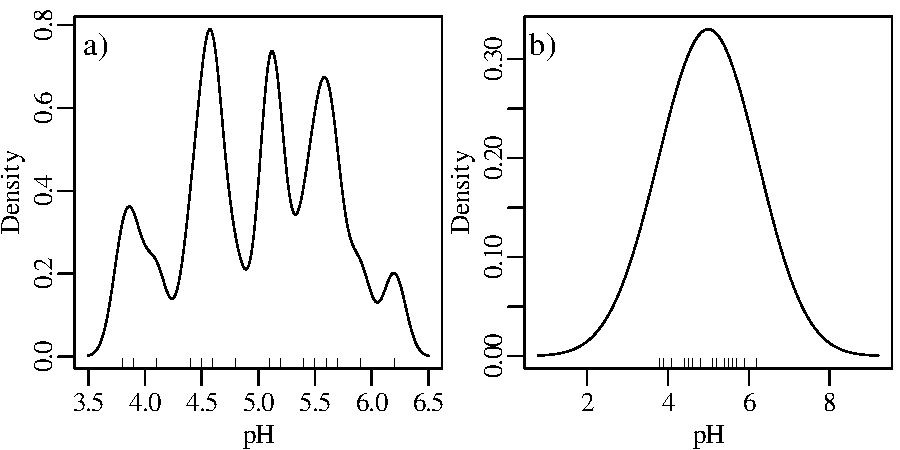
\includegraphics[width=\textwidth]{../figures/bandwidth.pdf}\medskip
\end{minipage}
\begin{minipage}[t][][t]{.45\textwidth}
  \captionof{figure}{KDEs of the pH data with a) a kernel bandwidth of
    $h=0.1$; and b) a bandwidth of $h=1$. Using a narrow bandwidth
    undermooths the data, whereas a wide bandwidth produces an
    oversmoothed distribution.}
\end{minipage}

Bandwidth selection is a similar problem to bin width selection.  A
deeper discussion of this problem falls outside the scope of text.
Suffice it to say that most statistical software (including $R$) use
equivalent rules of thumb to Sturges' Rule to set the bandwidth.  But
these values can be easily overruled by the user.

\section{Data transformations}
\label{sec:transformations}

Consider the following dataset of 20 measurements of sedimentary
clast sizes, in centimetres:

\begin{center}
0.35, 11.00, 6.00, 1.80, 2.30, 0.59, 8.40, 2.90, 5.90, 2.10,\\
1.20, 2.10, 1.10, 1.60, 0.90, 1.70, 3.40, 0.53, 2.20, 7.70
\end{center}

\noindent\begin{minipage}[t][][b]{.3\textwidth}
  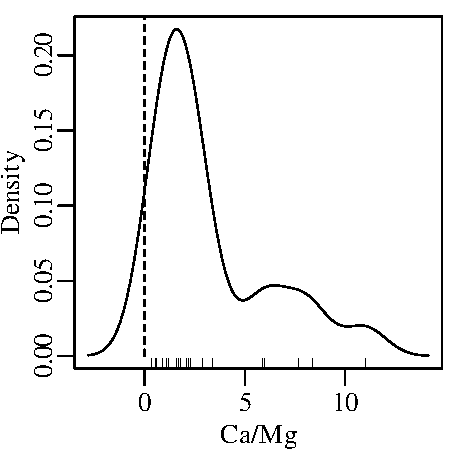
\includegraphics[width=\textwidth]{../figures/negativeKDE.pdf}\medskip
\end{minipage}
\begin{minipage}[t][][t]{.7\textwidth}
  \captionof{figure}{KDE of 20 clast size measurements.  Even though
    all the measurements are strictly positive, the curve extends into
    negative data space.}
  \label{fig:negativeKDE}
\end{minipage}

Clast sizes are strictly positive values. Yet the left tail of the KDE
extends into negative data space, implying that there is a finite
chance of observing negative sizes.  This is clearly nonsense.  In
geophysics, positive quantities are sometimes called \emph{Jeffreys
  quantities} (so named after the British geophysicist Sir Harold
Jeffreys). In addition to length, other examples of Jeffreys
quantities are mass, volume, density, speed, etc. These parameters
exist within an infinite half space between 0 and $+\infty$. We can
transform them to the entire infinite space of numbers by applying a
logarithmic transformation:\medskip

\noindent\begin{minipage}[t][][b]{.6\textwidth}
  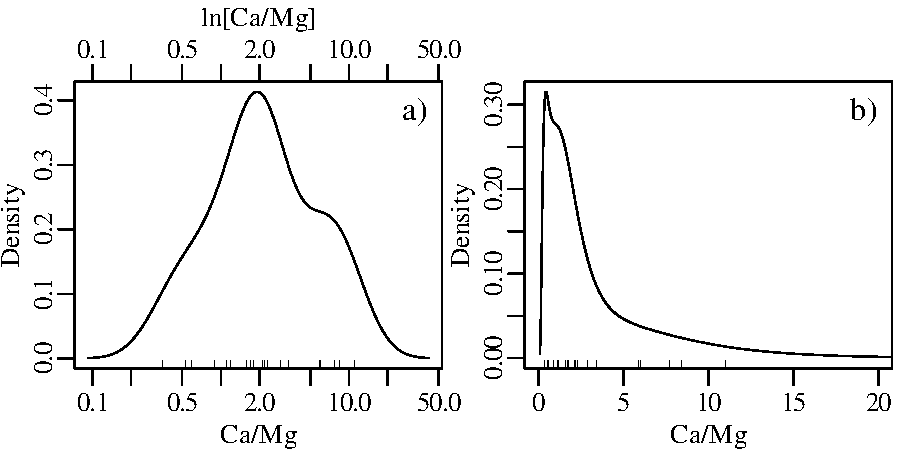
\includegraphics[width=\textwidth]{../figures/logKDE.pdf}\medskip
\end{minipage}
\begin{minipage}[t][][t]{.4\textwidth}
  \captionof{figure}{a) KDE of the clast size measurements, after
    applying a (natural) logarithmic transformation.  Note how the
    distribution has become more symmetric compared to the linear
    scale of Figure~\ref{fig:negativeKDE}. b) The same KDE mapped back
    to linear scale. Unlike Figure~\ref{fig:negativeKDE}, the mapped
    distribution does not cross over into negative values.}
  \label{fig:logKDE}
\end{minipage}

Jeffreys quantities are just one example of constrained measurements.
As another example, consider the following twenty porosity
measurements in limestone:\medskip

\begin{center}
  5.8, 28.0, 12.0, 27.0, 40.0, 12.0, 3.8, 6.3, 17.0, 16.0,\\
  95.0, 94.0, 92.0, 88.0, 88.0, 70.0, 92.0, 72.0, 74.0, 84.0
\end{center}

Porosity takes on values between 0 and 1 (if expressed as fractions,
or between 0 and 100 if expressed as percentages). Yet again the
Gaussian KDE of the data plot into physically impossible values of
$<0$ and $>1$:\medskip

\noindent\begin{minipage}[t][][b]{.3\textwidth}
  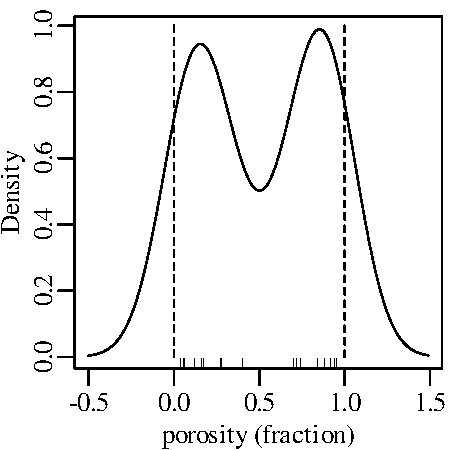
\includegraphics[width=\textwidth]{../figures/porosityKDE.pdf}\medskip
\end{minipage}
\begin{minipage}[t][][t]{.7\textwidth}
  \captionof{figure}{KDE of 20 porosity measurements.  Even though all
    the measurements are between 0 and 1, the KDE extends beyond these
    hard limits.}
  \label{fig:porosityKDE}
\end{minipage}

Using a similar approach as before, the dataspace can be opened up
from the constraints of the 0 to 1 interval to the entire line of
numbers, from $-\infty$ to $+\infty$. For proportions, this is
achieved by the \emph{logistic transformation}:

\begin{equation}
  u = \mbox{logit}(x) = \ln\!\left[\frac{x}{1-x}\right]
  \label{eq:logit}
\end{equation}

After constructing the density estimate (or carrying out any other
numerical manipulation), the results can be mapped back to the 0 to 1
interval with the inverse logit transformation:

\begin{equation}
  x = \mbox{logit}^{-1}(u) = \frac{\exp[u]}{\exp[u]+1}
  \label{eq:invlogit}
\end{equation}

\noindent\begin{minipage}[t][][b]{.6\textwidth}
  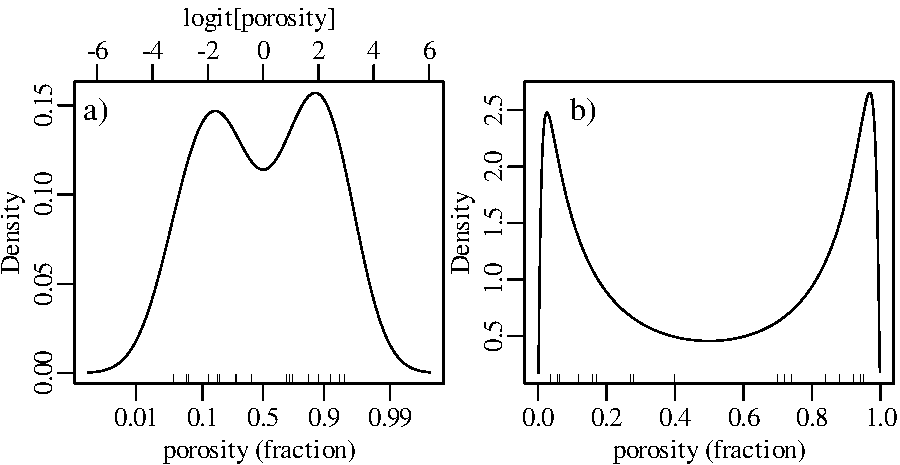
\includegraphics[width=\textwidth]{../figures/logitKDE.pdf}\medskip
\end{minipage}
\begin{minipage}[t][][t]{.4\textwidth}
  \captionof{figure}{a) KDE of the porosity data, after applying a
    logistic transformation.  Note the two horizonal axes.  The top
    axis marks the transformed values on a linear scale that extends
    from $-\infty$ to $+\infty$. The bottom axis is labeled by the
    actual porosity values on a non-linear scale that extends from 0
    to 1. b) The same distribution mapped back to the 0 -- 1
    interval.}
  \label{fig:logitKDE}
\end{minipage}

We will see in chapter~\ref{ch:compositional} that the logistic
transformation is a special case of a general class of \emph{logratio
  transformations} that are useful for the analysis of
\emph{compositional data}.

\section{Multivariate distributions}
\label{sec:multivariate}

KDEs can be generalised from one to two dimensions.  For example,
consider a dataset of eruption timings from the Old Faithful geyser in
Yellowstone national park (Wyoming, USA): \medskip

\noindent\begin{minipage}[t][][b]{.5\textwidth}
  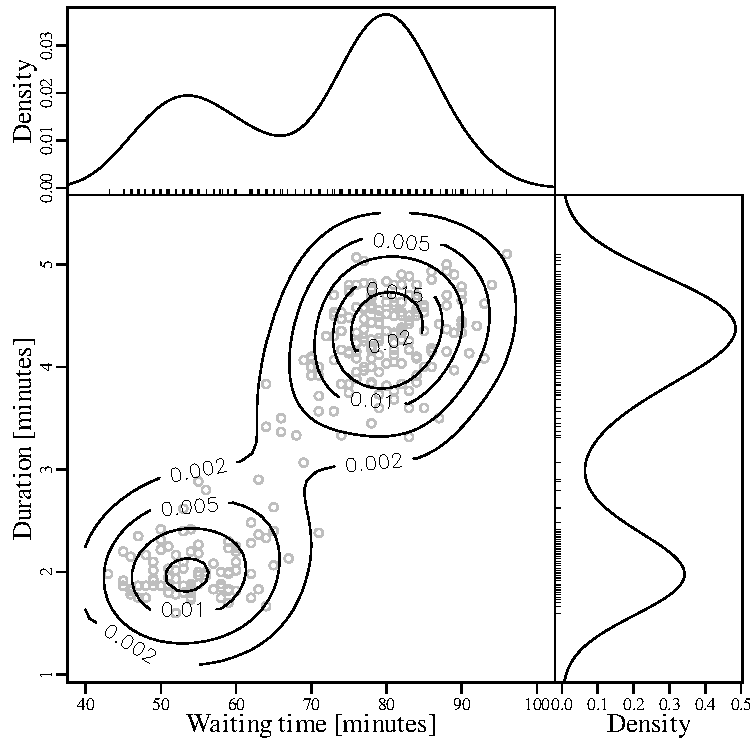
\includegraphics[width=\textwidth]{../figures/KDE2D.pdf}\medskip
\end{minipage}
\begin{minipage}[t][][t]{.5\textwidth}
  \captionof{figure}{Old Faithful eruption measurements. The dataset
    records 272 observations of 2 variables: the duration of each
    eruption, and the waiting time between them. Both variables are
    expressed in minutes. The lower left panel shows the bivariate
    measurements as grey circles. The contour lines represent a
    2-dimensional KDE. The marginal distributions of the waiting times
    (top) and eruption durations (right) are shown as 1-dimensional
    KDEs.}
  \label{fig:KDE2D}
\end{minipage}

It is generally not possible to visualise datasets of more than two
dimensions in a single graphic. In this case there are two options:

\begin{enumerate}
  \item plot the data as a series of 1- or 2-dimensional marginal
    plots; or
  \item extract the most important patterns or trends in the data by
    projection onto a lower dimensional plane. Then show these
    projected data as a lower dimensional graphic.
\end{enumerate}

The second strategy is also known as ``ordination'' and will be
discussed in detail in section~\ref{sec:PCA}.

\section{Empirical cumulative distribution fuctions}
\label{sec:ECDF}

Both histograms and kernel density estimates require the selection of
a `smoothing parameter'. For the histogram, this is the bin width; for
the KDE, it is the bandwidth. Despite the existence of rules thumbs to
automatically choose an appropriate value for the smoothing parameter,
there nevertheless is a level of arbitrariness associated with
them. The empirical cumulative distribution function (ECDF) is an
alternative data visualisation device that does not require
smoothing. An ECDF is step function that jumps up by $1/n$ at each of
$n$ data points.  The mathematical formula for this procedure can be
written as:
  
  \begin{equation}
    F(x) = \sum\limits_{i=1}^{n} 1(x_i<x)/n
    \label{eq:ECDF}
  \end{equation}
 
\noindent where $1(\ast) = 1$ if $\ast$ is `true' and $1(\ast) = 0$ if
$\ast$ is `false'. The y-coordinates of the ECDF are values from 0 to
1 that mark the fraction of the measurements that are less than a
particular value.  Plotting the pH, clast size, porosity and geyser
data as ECDFs:

\noindent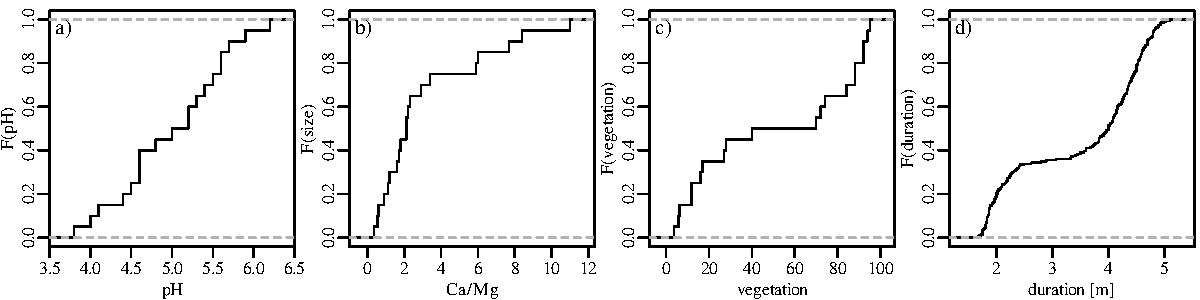
\includegraphics[width=\textwidth]{../figures/ECDFs.pdf}
\begingroup
\captionof{figure}{Empirical cumulative distribution functions (ECDFs)
  of, from left to right: a) the pH data (whose KDE is shown in
  Figure~\ref{fig:pHgaussKDE}); b) the clast size data of
  Figure~\ref{fig:negativeKDE}; c) the porosity data of
  Figure~\ref{fig:porosityKDE}; and d) the eruption time data of
  Figure~\ref{fig:KDE2D}. Note that ECDFs are only applicable to
  1-dimensional datasets.\medskip}
\label{fig:ECDFs}
\endgroup

ECDFs do not require binning or selecting a bandwidth.  Because they
do not require smoothing, they do not spill over into physically
impossible values for the clast size and porosity data. Therefore the
construction of an ECDF is completely hands off.\medskip

The visual interpetation of ECDFs is different from that of histograms
or KDEs. Whereas different clusters of values stand out as `peaks' in
a histogram or KDE, they are marked by steep segments of the ECDF. For
example, the two peaks in the KDE of the geyser data
(Figure~\ref{fig:KDE2D}) correspond to two steps in the ECDF
(Figure~\ref{fig:ECDFs}.d).
